\subsection{Whitened Stochastic Variational Gaussian Processes}
\label{sec:variational_results}

As a first application, we will demonstrate that the CIQ whitening procedure $\bK^{-1/2} \bb$ can increase the fidelity of {\bf stochastic variational Gaussian processes (SVGP)} \cite{hensman2013gaussian,hensman2015scalable,matthews2017scalable}.
%The whitening operation is commonly used with variational approximations to accelerate the learning of variational parameters.
%
%\paragraph{Stochastic variational Gaussian process inference}
These models are used for non-conjugate likelihoods (e.g. GP classification) or for large datasets that do not fit into memory.
As described in \cref{sec:variational}, SVGP forms an approximate posterior
\[
  p(f(\bx) \mid \bX, \by) \approx q(f(\bx)) = \Evover{q(\bu)}{ p\left( f(\bx) \mid \bu \right)},
\]
where $\bu \in \reals^M$ are {inducing function values}.
$q \left( \bu \right)$ is a variational Gaussian distribution parameterized by mean $\bmm \in \reals^M$ and covariance $\bS \in \reals^{M \times M}$.
$\bmm$ and $\bS$ (as well as the model's kernel/likelihood hyperparameters) are chosen to optimize the variational ELBO:
%
\begin{align*}
  -\loglik_\text{ELBO}\Bigl\{ \bmm, \bS \Bigr\} &= -\sum_{i=1}^N \Evover{q(f(\bx^{(i)}))}{  \: \log p( y^{(i)} \mid f(\bx^{(i)}) ) \: } + \kl{ q(\bu) }{ p(\bu) }.
\end{align*}
As stated in \cref{sec:variational}, the ELBO factorizes over all data points in the training set $\bX, \by$.
Therefore, it can be approximated using minibatches and used in conjunction with stochastic gradient optimization.

Rather than directly learning $\bmm$ and $\bS$, it is more common to learn the \emph{whitened parameters} \cite{kuss2005assessing,matthews2017scalable}:
$ \bmm' = \bK_{\bZ\bZ}^{- 1/ 2} \bmm$ and $\bS' = \bK_{\bZ\bZ}^{-1 / 2} \bS \bK_{\bZ\bZ}^{-1 / 2}. $
Under these coordinates, the KL divergence term is
\[ \frac{1}{2} ( \bmm^{\prime \top} \bmm' + \tr{ \bS' } - \log \vert \bS' \vert - M ),\]
%
which doesn't depend on $p(\bu)$ and therefore is relatively simple to optimize.
The posterior distribution $q(f(\bx)) = \normaldist{\ameantest{\bx}}{\avartest{\bx}}$ is given by
%
\begin{equation}
  \begin{split}
  \ameantest{\bx} &= \bk_{\bZ\bx}^\top \bK_{\bZ\bZ}^{-\frac 1 2} \bmm',
  \\
  \avartest{\bx} &= k(\bx, \bx) -
    \bk_{\bZ\bx}^\top \bK_{\bZ\bZ}^{-\frac 1 2} \left( \bI - \bS' \right) \bK_{\bZ\bZ}^{-\frac 1 2} \bk_{\bZ\bx}.
  \end{split}
  \label{eqn:approx_pred_dist}
\end{equation}

\paragraph{Time and space complexity.}
During training, we repeatedly compute the ELBO and its derivative, which requires computing \cref{eqn:approx_pred_dist} and its derivative for a minibatch of data points.
Optimization typically requires up to $10,\!000$ iterations of training \citep[e.g.][]{salimbeni2018natural}.
We note that $\bK_{\bZ\bZ}^{-1 / 2} \bb$ (and its derivative) is the most expensive numerical operation during each ELBO computation.
If we use Cholesky to compute this operation, the time complexity of SVGP training is $\bigo{M^3}$.
On the other hand, CIQ-based SVGP training is only $\bigo{J M^2}$, where $J$ is the number of msMINRES iterations.
Both methods require $\bigo{M^2}$ storage for the $\bmm'$ and $\bS'$ parameters.

\paragraph{Natural gradient descent with CIQ.}
The size of the variational parameters $\bmm'$ and $\bS'$ grows quadratically with $M$.
This poses a challenging optimization problem for standard gradient descent methods.
To adapt to this parameter increase, we rely on {\bf natural gradient descent (NGD)} to optimize $\bmm'$ and $\bS'$ \citep[e.g.][]{hensman2012fast,salimbeni2018natural}.
At a high level, these methods perform the updates $[\bmm, \:\: \bS] \gets [\bmm, \:\: \bS] - \varphi \: \bFS^{-1} \: \nabla \loglik_\text{ELBO}$,
where $\varphi$ is a step size, $\nabla \loglik_\text{ELBO}$ is the ELBO gradient, and $\bFS$ is the {Fisher information matrix} of the variational parameters.
%\citet{salimbeni2018natural} find that NGD updates on $\bmm'$ and $\bS'$ allow for faster optimization than single-order optimizers.
%
Na\"ively, each NGD step requires $\bigo{M^3}$ computations with $\bmm'$ and $\bS'$ which would dominate the cost of CIQ-based SVGP.
Fortunately, we can derive a natural gradient update that only relies on matrix solves with $\bS'$, which take $\bigo{J M^2}$ time using preconditioned conjugate gradients.
Therefore, using NGD incurs the same \emph{quadratic} asymptotic complexity as CIQ-SVGP.
See \cref{app:ngd} for the $\bigo{M^2}$ NGD update equations.

\paragraph{Comparison of Cholesky vs CIQ.}
We compare CIQ verses Cholesky for computing \cref{eqn:approx_pred_dist} when training SVGP models.\footnote{
  Note that Cholesky computes $\bK^{-1/2} \bb$ up to an orthogonal rotation, which is suitable for whitened SVGP.
}
We test on 3 large-scale spatial datasets: a GIS dataset ({\bf 3droad}, $D=2$), a monthly precipitation dataset ({\bf Precipitation}, $D=3$), and a tree cover dataset ({\bf Covtype}, $D=54$).
Each task has between $N=70,\!000$ and $N=500,\!000$ training data points.
For 3droad we use a Gaussian observation model.
The Precipitation dataset has noisier observations; therefore we apply a Student-T observation model.
Finally, we reduce the CovType dataset to a binary classification problem and apply a Bernoulli observation model.\footnote{
  The task is predicting whether the primary tree cover at a given location is pine trees or other types of trees.
}
We train models with $M$ ranging between $1,\!000$ to $10,\!000$.

\paragraph{Experimental Details.}
Each dataset is randomly split into $75\%$ training, $10\%$ validation, and $15\%$ testing sets; $\bx$ and $y$ values are scaled to be zero mean and unit variance.
All models use a constant mean and a Mat\'ern 5/2 kernel, with lengthscales initialized to $0.01$ and inducing points initialized by $K$-means clustering.
Each model is trained for $20$ epochs with a minibatch size of $256.$\footnote{
  The batch size is $512$ on the Covtype dataset due to its larger size.
}
We alternate between optimizing $\bmm'/\bS'$ and the other parameters, using natural gradient descent for the former and Adam \cite{kingma2014adam} for the latter.
Each optimizer uses an initial learning rate of $0.01$\footnote{
  On the Precipitation dataset, we use an initial learning rate of $0.005$ for  NGD stability with the Student-T likelihood.
}, decayed by $10\times$ at epochs $1$, $5$, $10$, and $15$.
For CIQ we use $Q = 15$ quadrature points.
MINRES terminates when the $\bc_j$ vectors achieve a relative norm of $0.001$ or after $J=200$ iterations.

%\paragraph{Training time.}
%In \cref{fig:variational_timing_and_stats} (left) we plot the training time (in hours) of CIQ/Cholesky models as a function of $M$.
%Each model is trained for $20$ epochs on a single NVIDIA Titan-RTX GPU.
%Both the Cholesky and CIQ variants take increasingly longer to train as $M$ increases.
%Nevertheless, we observe that CIQ models are able to scale to larger $M$ values under a fixed computational budget.
%Both CIQ and Cholesky take roughly the same amount of time for $M=1,\!000$ inducing points.
%However, CIQ models are roughly $4\times$ faster at $M=5,\!000$.
%On the Precipitation dataset, a CIQ model with $M=10,\!000$ finishes training faster than a Cholesky model with $M=5,\!000$.

\begin{figure}[t!]
  \centering
  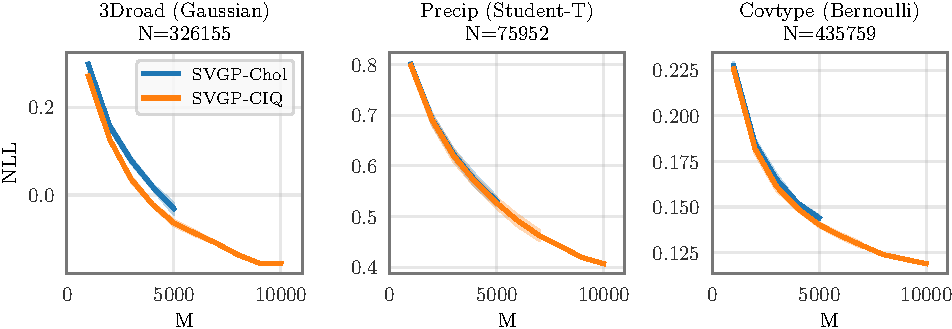
\includegraphics[width=\linewidth]{figures/variational_nll.pdf}
  \caption[Negative log likelihood (NLL) comparison of Cholesky-whitened vs CIQ-whitened SVGP models.]{
    Negative log likelihood (NLL) comparison of Cholesky vs CIQ SVGP models.
    {\bf Left:} 3DRoad dataset ($N=326155, D=2$, Gaussian likelihood).
    {\bf Middle:} Precipitation dataset ($N=75952, D=3$, Student-T likelihood).
    {\bf Right:} CoverType dataset ($N=435759, D=54$, Bernoulli likelihood).
    NLL improves with inducing points ($M$); Cholesky and CIQ models have similar performance.
    However CIQ models train faster than their Cholesky counterparts.
  }
  \label{fig:variational_nll}
\end{figure}

\begin{figure}[t!]
  \centering
  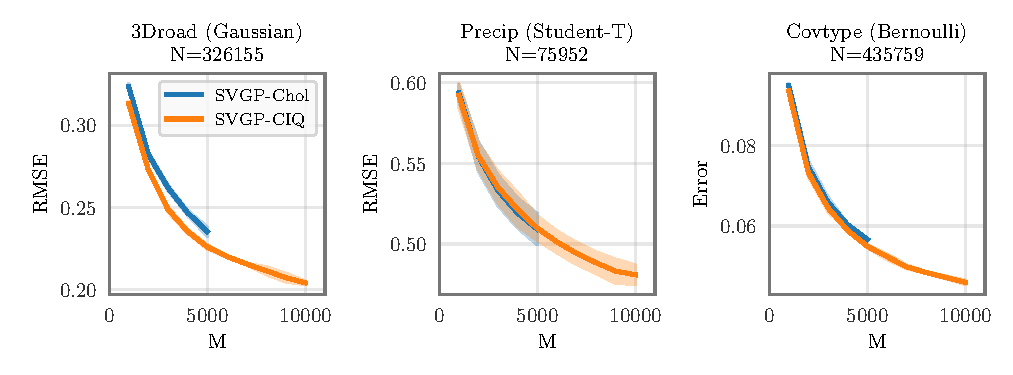
\includegraphics[width=\linewidth]{figures/variational_error.pdf}
  \caption[Error comparison of Cholesky-whitened vs CIQ-whitened SVGP models.]{
    Error comparison of Cholesky-whitened vs CIQ-whitened SVGP models.
    {\bf Left:} 3DRoad dataset RMSE ($N=326155, D=2$, Gaussian likelihood).
    {\bf Middle:} Precipitation dataset RMSE ($N=75952, D=3$, Student-T likelihood).
    {\bf Right:} CoverType dataset $0/1$ error ($N=435759, D=54$, Bernoulli likelihood).
  }
  \label{fig:variational_error}
\end{figure}

\paragraph{Results.}
The computations of $\bK_{\bZ\bZ}^{-1/2} \bk_{\bZ\bx}$ from CIQ and Cholesky are the same up to an orthogonal rotation.
However, adaptive gradient optimizers (which we use for the kernel/likelihood hyperparameters) are not invariant to orthogonal transformation.
While CIQ and Cholesky SVGP models may learn different parameters, the two methods achieve very similar test-set negative log likelihood (\cref{fig:variational_nll}) and predictive error (\cref{fig:variational_error}).
%On 3droad, CIQ models tend to slightly outperform Cholesky models.
The key difference is the training time:
with $M=5,\!000$ inducing points, CIQ models are up to \emph{5.6 times faster} than Cholesky models (as measured on a Titan RTX GPU).
Moreover, CIQ models with $M=8,\!000$-$10,\!000$ take roughly the same amount of time as $M=5,\!000$ Cholesky models.
We do not train $M > 5,\!000$ Cholesky models as such these would require $2$-$10$ days for training.

\begin{figure}[t!]
  \centering
  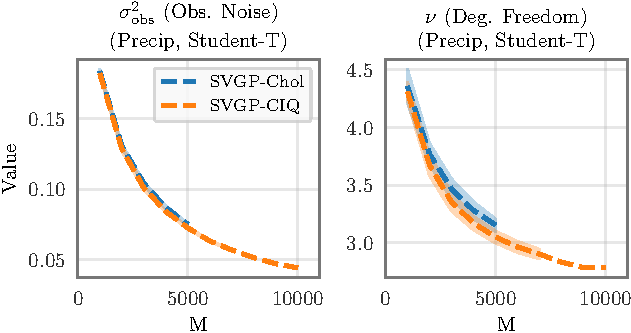
\includegraphics[width=\linewidth]{figures/variational_stats.pdf}
  \caption[Train time comparison of Cholesky-whitened vs CIQ-whitened SVGP models.]{
    Hyperparameters verses number of inducing points ($M$) for Chol-SVGP and CIQ-SVGP (Precipitation dataset, Student-T likelihood).
    As $M$ increases, the kernel outputscale (left) also increases.
    At the same time, the estimated observational noise (middle) decreases as does the estimated degrees of freedom (right), reflecting a heavier-tailed noise distribution.
    This suggests that, with larger $M$, SVGP models can find more signal in the data.
  }
  \label{fig:variational_stats}
\end{figure}

\paragraph{Effects of increased inducing points.}
We find that accuracy improves with increased $M$ on all datasets.
Scaling from $M=5,\!000$ to $M=10,\!000$ reduces test-set NLL by $0.1$ nats on the 3droad and Precipitation datasets.
We find similar reductions in predictive error (\cref{fig:variational_error} for plots).
By scaling more readily to large $M$, CIQ enables high-fidelity variational approximations that would be computationally prohibitive with Cholesky.

We also find that increasing $M$ changes the values of the learned kernel/likelihood hyperparameters.
In \cref{fig:variational_stats} we plot the learned hyperparameters of the Precipitation SVGP models:
%
\begin{enumerate*}
  \item $o^2$ (the kernel outputscale)---which roughly corresponds to variance explained as ``signal'' in the data;
  \item $\sigma^2_\text{obs}$---which roughly corresponds to variance explained away as observational noise; and
  \item $\nu$ (degrees of freedom)---which controls the tails of the noise model (lower $\nu$ corresponds to heavier tails).
\end{enumerate*}
%
As $M$ increases, we find that the observational noise parameter decreases by a factor of $4$---down from $0.19$ to $0.05$---while the $\nu$ parameter also decreases.
Models with larger $M$ values can more closely approximate the true posterior \cite{hensman2013gaussian}; therefore, we expect that the larger-$M$ likelihoods more closely correspond to the true parameters.
This confirms findings from \citet{bauer2016understanding}, who argue that variational approximations with small $M$ tend to overestimate the amount of noise in datasets.
